% Valentino Vranic
% Metody inzinierskej prace 2012/13

\documentclass{beamer}

%\usetheme{Warsaw}
%\usetheme{Antibes}
\usetheme{Darmstadt}
%\usetheme{Goettingen}

\usecolortheme{default}
%\usecolortheme{dolphin}
%\usecolortheme{rose}
% http://deic.uab.es/~iblanes/beamer_gallery/index_by_color.html
%\usecolortheme{beaver}

%\useoutertheme[]{sidebar}

\setbeamercovered{transparent}

\usepackage[english]{babel}
\usepackage[T1]{fontenc}
\usepackage[utf8]{inputenc}
\usepackage{url}

\usepackage{listings}

\lstset{language=C++,basicstyle=\fontsize{8}{9.6}\selectfont,showstringspaces=false,columns=fullflexible,identifierstyle=\ttfamily,keywordstyle=\bfseries,showstringspaces=false,columns=fullflexible}
%\lstset{language=C,basicstyle=\fontsize{10.5}{12.6}\selectfont,identifierstyle=\ttfamily,keywordstyle=\bfseries,showstringspaces=false,columns=fixed}

\def\BibTeX{\textsc{Bib}\kern-.08em\TeX} 

\newcommand{\footcite}[1]{\footnote{\tiny #1}}
\newcommand{\umlet}{.5}
\newcommand{\emp}[1]{\textit{\alert{#1}}}
\newcommand{\kw}[1]{\mbox{\textbf{#1}}}
\newcommand{\id}[1]{\texttt{#1}}
\newcommand{\stl}{\guillemotleft}
\newcommand{\str}{\guillemotright}

\newcommand{\lsti}{\lstinline[basicstyle=\fontsize{10.5}{12.1}\selectfont]}

\newcommand{\ssection}[1]{
	\section{#1}
	\begin{frame}[fragile=singleslide]\frametitle{}
	\Huge #1
	\end{frame}
}

\newcommand{\ssectionn}[1]{
	\section*{#1}
	\begin{frame}[fragile=singleslide]\frametitle{}
	\Huge #1
	\end{frame}
}

\newenvironment{program}{\begin{beamercolorbox}[rounded=true,shadow=true]{block body}\vspace{-4mm}}{\vspace{-2mm}\end{beamercolorbox}}

\setbeamercolor{fvystup}{fg=white,bg=black}
\newenvironment{vystup}{\begin{beamercolorbox}[rounded=true,shadow=true]{fvystup}}{\end{beamercolorbox}}

\newenvironment{poznamka}{\begin{beamercolorbox}[rounded=true,shadow=false]{block body}}{\end{beamercolorbox}}

\setbeamertemplate{footline}[page number]
{
%\insertpagenumber
%\begin{beamercolorbox}{section in head/foot}
%\vskip2pt\insertnavigation{\paperwidth}\vskip2pt
%\end{beamercolorbox}%
}



\author{Tomáš Brček}
%\url{www.fiit.stuba.sk/~vranic}, \url{vranic@fiit.stuba.sk}}
%{\tiny \url{www.fiit.stuba.sk/~vranic}, \url{vranic@fiit.stuba.sk}}

\subtitle{\vspace{3mm} Metódy inžinierskej práce 2022/2023}

\title{Teaching mathematics through games in primary schools (grades 1-3)
}

\date{\footnotesize 22. november 2022}




\begin{document}

\begin{frame}[fragile=singleslide]
\titlepage
\end{frame}


\begin{frame}[fragile=singleslide]\frametitle{Contents}
\begin{itemize}
\item Why did I choose this topic?
\item Introduction
\item Related work
\item Game-based learning
\item How often do primary teachers use games to support mathematics instruction?
\item World programs
\item Conclusion
\end{itemize}
\end{frame}


\begin{frame}[fragile=singleslide]\frametitle{}
Why did I choose this topic?
\end{frame}


\section{}
% príkaz \ssection by vytvoril zvláštný slajd s názvom časti - v krátkych prezentáciách to prekáža, lebo oberá o čas

\begin{frame}[fragile=singleslide]\frametitle{Introduction}
\begin{itemize}
\item mathematics and games
\item technologies
\item students are changing
\item Is it really beneficial?
\item impact on motivation
\end{itemize}
\end{frame}



\section{}

\begin{frame}[fragile=singleslide]\frametitle{How often do primary teachers use games to support mathematics instruction?}
\begin{table} [hbtp]
    \caption{Frequency Teachers Reported Playing Mathematical Games}
    \label{tab:table1}
    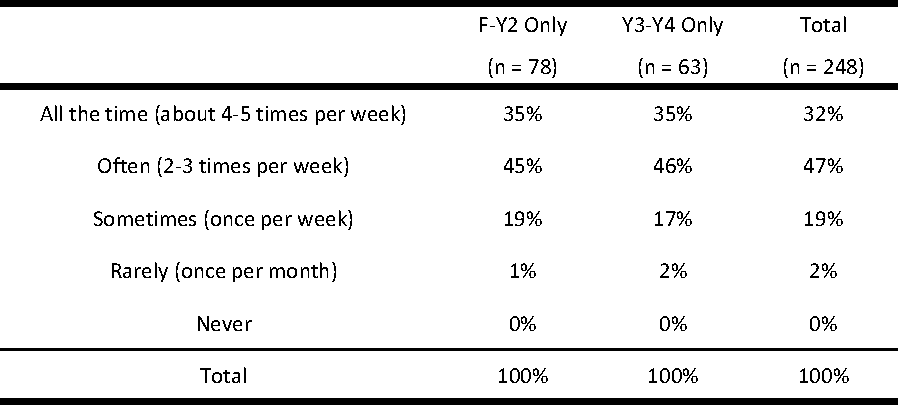
\includegraphics[width=\textwidth]{table1-crop}
\end{table}
\end{frame}


\begin{frame}[fragile=singleslide]\frametitle{World programs}
\begin{figure}[h]
    \centering
    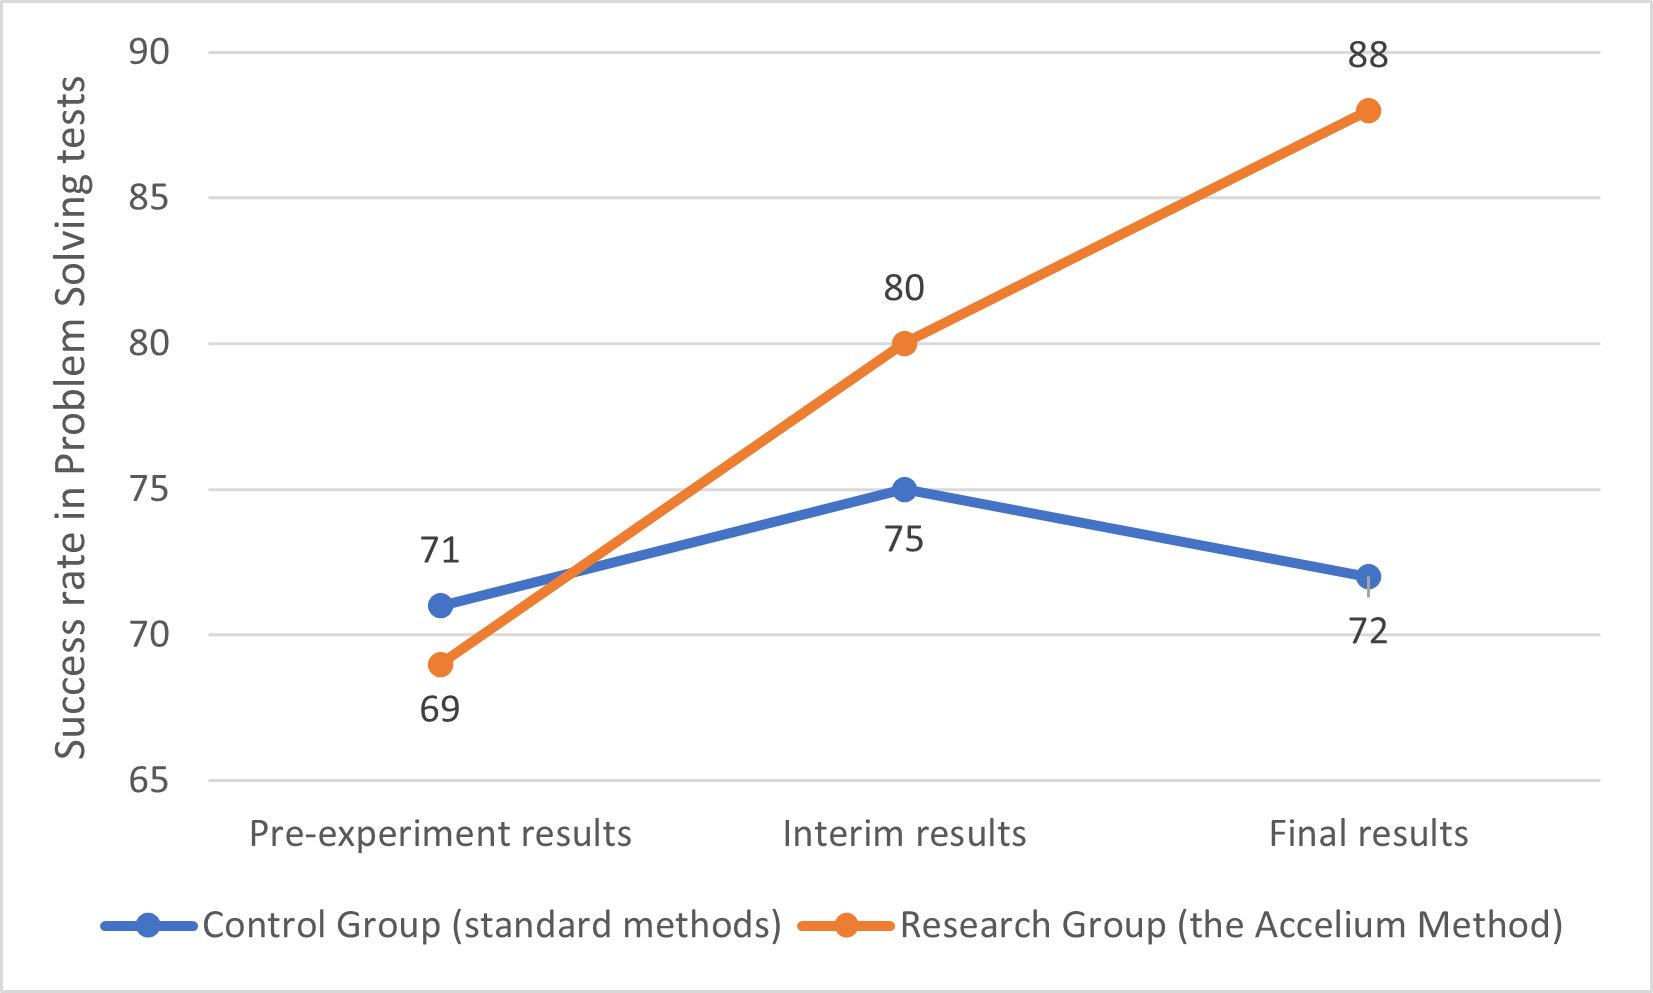
\includegraphics[width=\textwidth]{accelium_graph}
    \caption{The Accelium Method \& Problem Solving}
    \label{fig:figure2}
\end{figure}
\end{frame}



\end{document}




Text \end{document} za príkazom \end{document} LaTeX ignoruje, takže tu môžete odkladať veci (aj celé slajdy), ktoré nechcete vymazať, lebo ich ešte možno budete potrebovať, avšak ich v danom momente nechcete mať v slajdoch.
